\documentclass[a4paper, 12pt, oneside]{Project}
\usepackage[utf8]{inputenc}

\title       {Automatic registration of multiple kinect in indoor environment.}
\UNIVERSITY  {UNIVERSITAT POLITÈCNICA DE CATALUNYA}
\supervisor  {Joan Aranda}
\examiner    {}
\degree      {Master's degree in Automatic Control and Robotics}
\authors     {Stéphane Maillot}
\department  {Department of Systems Engineering, Automation \\ and Industrial Informatics}
\faculty     {Barcelona School of Industrial Engineering}



\usepackage{graphicx}
\graphicspath{ {images/} }
% \usepackage[backend=bibtex,style=verbose-trad2]{biblatex}

\usepackage[acronym]{glossaries}
\makeglossaries
\newglossaryentry{middleware}
{
        name=middleware,
        description={Computer software that provides services to software applications beyond those available from the operating system}
}
\newglossaryentry{open source}
{
        name=open source,
        description={Software which source code is free to access and redistribute to encourage peer production and knowledge sharing}
}
\newglossaryentry{library}
{
        name=library,
        description={Collection of resources used by computer programs to gain behaviors implemented inside that library with to implement that behavior itself}
}
\newglossaryentry{intrinsic}
{
        name=intrinsic calibration,
        description={Calibration of the camera that consists in finding parameters that depends only on the device like focal length, focal center, deformation matrix etc. This calibration is required for \glslink{extrinsic}{extrinsic} calibration}
}
\newglossaryentry{extrinsic}
{
    name=extrinsic calibration,
    description={Calibration of the camera that consists in finding the position of the camera in its environment}
}

\newglossaryentry{rosnode}
{
    name=ROS node,
    description={In \acrshort{ros} framework, a node is a process that perform some computation and communicate with other nodes. A program is composed by a combination of nodes}
}
\newacronym{icp}{ICP}{Iterative Closest Point}
\newacronym{ar}{AR}{Augmented Reality}
\newacronym{iss}{ISS}{Intrinsic Shape Signature}
\newacronym{narf}{NARF}{}

\begin{document}

\maketitle

% #############################################################################

% It is better to have smaller font and larger 
% line spacing than the other way round
\setstretch{1.3}  

% Define the page headers using the FancyHdr 
% package and set up for one-sided printing
\fancyhead{}      % Clears all page headers and footers
\rhead{\thepage}  % Sets the right side header to show the page number
\lhead{}          % Clears the left side page header
\pagestyle{fancy}  % Finally, use the "fancy" page style 

\bibliographystyle{plain}
\bibliography{references}
\addcontentsline{toc}{chapter}{Bibliography}


% #############################################################################
%                               The Abstract Page
% #############################################################################
\clearpage 
\lhead{\emph{Preface}}

% ***************************************************************************
\chapter*{Abstract}
\addcontentsline{toc}{chapter}{Abstract} 
% ***************************************************************************

This thesis presents how to register point clouds from RGB-D sensors to perform 3D reconstruction of an indoor scene. \\
Several techniques have been explored to find the most effective technique for our setup. 


% #############################################################################
%                                 CONTENTS
% #############################################################################
\clearpage 
\pagestyle{fancy} 
\lhead{\emph{Contents}}  
\tableofcontents 

\clearpage  
\pagestyle{empty}  

\mainmatter	  % Begin normal, numeric (1,2,3...) page numbering
\pagestyle{fancy}  % Return the page headers back to the "fancy" style

\lhead{\emph{Preface}}

% ***************************************************************************
\chapter*{Preface}
\addcontentsline{toc}{chapter}{Preface} 
% ***************************************************************************


% ***************************************************************************
\section*{Origin of the project}
\addcontentsline{toc}{section}{Origin of the project} 
% ***************************************************************************

Although robots have been used for decades in the industry, one of the current challenge for robotics is to adapt robots for domestic environment to help people in their everyday life. With this in mind, this project aims to teach robots how to interact with humans in a kitchen environment in order to help them achieving common actions in a collaborative way. This project particularly applies to disabled people who may need assistance for achieving daily tasks.   

% ***************************************************************************
\section*{Motivation}
\addcontentsline{toc}{section}{Motivation} 
% ***************************************************************************

To achieve this goal we need to acquire a detailed representation of the scene before being able to act on the environment with robots. Using computer vision to build a detailed and real-time 3D map of the scene in real time is then a necessary step to achieve in order for the robots to understand their environment before choosing a desired action and planning a trajectory to actually perform this task. This project use the kinect V2 depth sensor to acquire 3D data from the scene. Kinect sensors have a better accuracy at close range and then, even when it is feasible, it will not be the best idea to put the sensor far away from the workspace in order to acquire data from the whole environment with only one sensor. \\
Thus, it is preferable to reconstruct the scene from partial views of the environment to gain accuracy when the scene is too large to use only one close range camera. It is then needed to merge different views into one single complete representation of the workspace. The main motivation of this work is then to be able to reconstruct the complete 3D map in order for the robots to be able to understand their environment.

% ***************************************************************************
\section*{Requirements}
\addcontentsline{toc}{section}{Requirements}
% ***************************************************************************

This work mainly require depth sensors, we are using Kinect V2. These sensors provide an high frequency (default: 30 \acrshort{fps}) stream of \acrshort{rgb} and depth data which are converted into 3D colored Point Clouds. The computer needed to process this amount of data have to be powerful if we want to process it with high frequency. In this project we use a Titan X \acrshort{gpu} and i7 cores to process the data.\\
For the implementation, this work is entirely made using free \gls{open source} software. It is running on Linux \acrshort{os} using \acrshort{ros} \gls{middleware} and \gls{open source} \gls{libraries} (\acrshort{pcl}, openCV and other \acrshort{ros} libraries). 
\lhead{\emph{Introduction}}

% ***************************************************************************
\chapter{Introduction}
% ***************************************************************************

% ***************************************************************************
\section{Objectives}
% ***************************************************************************



% ***************************************************************************
\section{Scope}
% ***************************************************************************

 
\lhead{\emph{State of the Art}}

% ***************************************************************************
\chapter{State of the Art}
% ***************************************************************************


% ***************************************************************************
\section{Marker detection}
% ***************************************************************************

The registration technique currently used in this project is the detection of \acrshort{ar} marker in the color image. AR markers are black and white, grid-like patterns developped for augmented reality usage to detect easily a position in space from an RGB camera. \\
This detection is not very accurate but by repeating the process hundreds of time and averaging we can get a good estimation of the position of the cameras. An obvious drawback regarding our needs for this project is the involvement of the user and the equipment requirement. The user need to place a printed pattern into the overlapping region and no other work can be done while performing the registration. \\
To perform this registration we place the marker in the overlapping region so that both camera can be calibrated from this marker (fig. \ref{fig:ar_marker}). As we have already discussed, the overlapping region cannot be trusted due to its poor quality and small size. This can be solved by calibrating both cameras with a different marker position (in the middle of the camera view), these positions have now to be know if we want to match point clouds together. This is a high constraint both for the user to perform the calibration twice and the workspace to be designed such that we can easily move the marker in it while still knowing exactly the position of the marker. This is the reason we are searching for a more automatic registration process for this project. \\

\begin{figure}[h!]
    \centering
    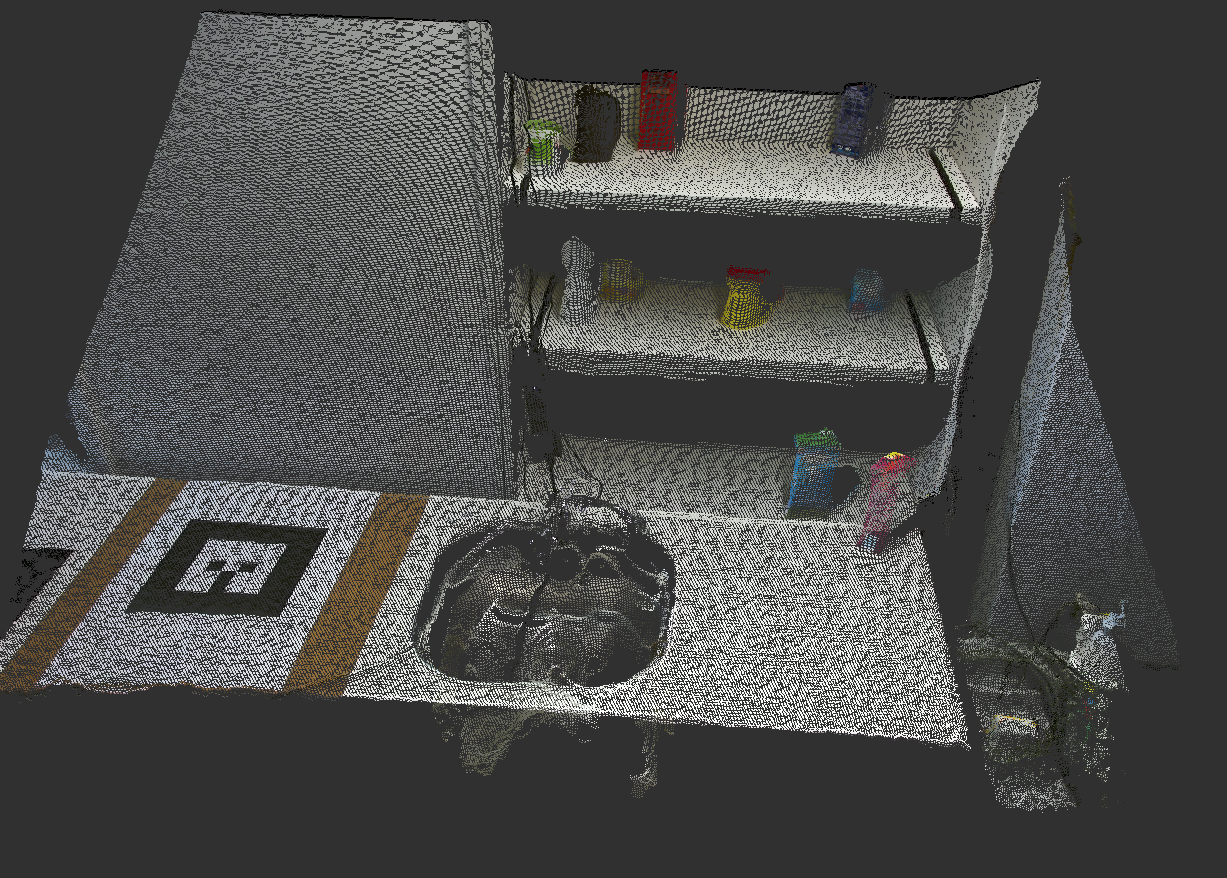
\includegraphics[width=\textwidth]{images/marker_detection.png}
    \caption{AR Marker detection.}
    \label{fig:ar_marker}
\end{figure}

For the implementation, we are using an existing ROS package based on alvar, which tracks AR printed patterns in a color image to estimate its position with respect to this camera. By filming a marker which position in the scene is known with a fix camera, we can average the pose estimation on hundreds of frames to get a good estimation of the actual position of the camera. \\
The main drawback of this technique are the need of printed pattern, human action, time of computation and knowledge of the scene. This is still a good technique to establish our ground truth and to build the entire scene point cloud we could need for other methods as ICP.


% ***************************************************************************
\section{\acrlong{icp}}
% ***************************************************************************

The \acrlong{icp} algorithm is a well known registration algorithm that aims to register 2 point clouds that represent the same objects using an iterative process. These iterations rely on identifying closest points from both point clouds at each step in order to estimate a transformation that will improve the clouds matching without taking account of distant points (considered as outliers).\\

The first step of this algorithm is to find matches between points from the source point cloud $\mathcal{P_S}$ to points in the target cloud $\mathcal{P_T}$. As we have no knowledge of which point within the target cloud should match with source points the key idea is to match source points with their closest neighbors in the target cloud (fig. \ref{fig:closest_point}). After filtering duplicate matches we have pairs of matching points with indices $m_S$ and $m_T$. At this step we define the objective function $f$ which is the \acrshort{mse} of these matches according to the current guess for the rigid transform $\mathcal{T}_{i}$. \\
\[
    f(\mathcal{T}_i) = MSE(\mathcal{P}_T^{m_T} - \mathcal{T}_i\: \mathcal{P}_S^{m_S})
\]
Where the initial guess $\mathcal{T}_0$ should be provided to the program, the quality of this guess will affect the final result. \\
After that we can compute the transform that minimize $f$ for this set of matches. Having a new estimation of the rigid transform, we can repeat the process until convergence. 

\begin{figure}[h!]
    \centering
    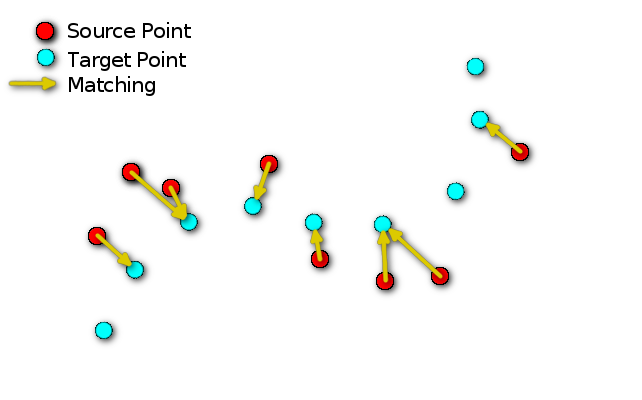
\includegraphics[width=\textwidth]{images/closest_point.png}
    \caption{ICP closest point matching.}
    \label{fig:closest_point}
\end{figure}

The main drawback of this technique come from the need of an initial guess, the \acrshort{icp} algorithm is used for refinement once we have a rough idea of the desired result. This is a problem in our case because we have no previous knowledge over the camera positions and orientation. It could be fixed by using accelerometers for example but the translation part would need a large overlapping region to be solved. This algorithm is indeed highly sensitive to the ratio of overlapping between point clouds. In our case, the low overlapping makes this techniques unusable, even if the registration converge to a coherent result (small translation error), the lack of overlapping, the noise and deformation would not allow to have an accurate estimation of the rotation between clouds which have dramatic effect on low-overlapping point clouds (2 sets of points with a similar centroids would be much less affected by rotation errors). \\
To perform registration using the ICP method, I am using the PCL implementation of this algorithm. As expected, applying this algorithm with our 2 low overlapping point clouds ends up to really bad results (fig. \ref{fig:icp_cams}), however this technique is really effective when registering a partial view of the scene with a complete model of it. I was then able to apply ICP to both point clouds to register them to a more complete 3D model of the scene. This works both when applied to registration with a CAD model of the kitchen and to a complete point cloud generated by merging both kinect views. \\

\begin{figure}[h!]
    \centering
    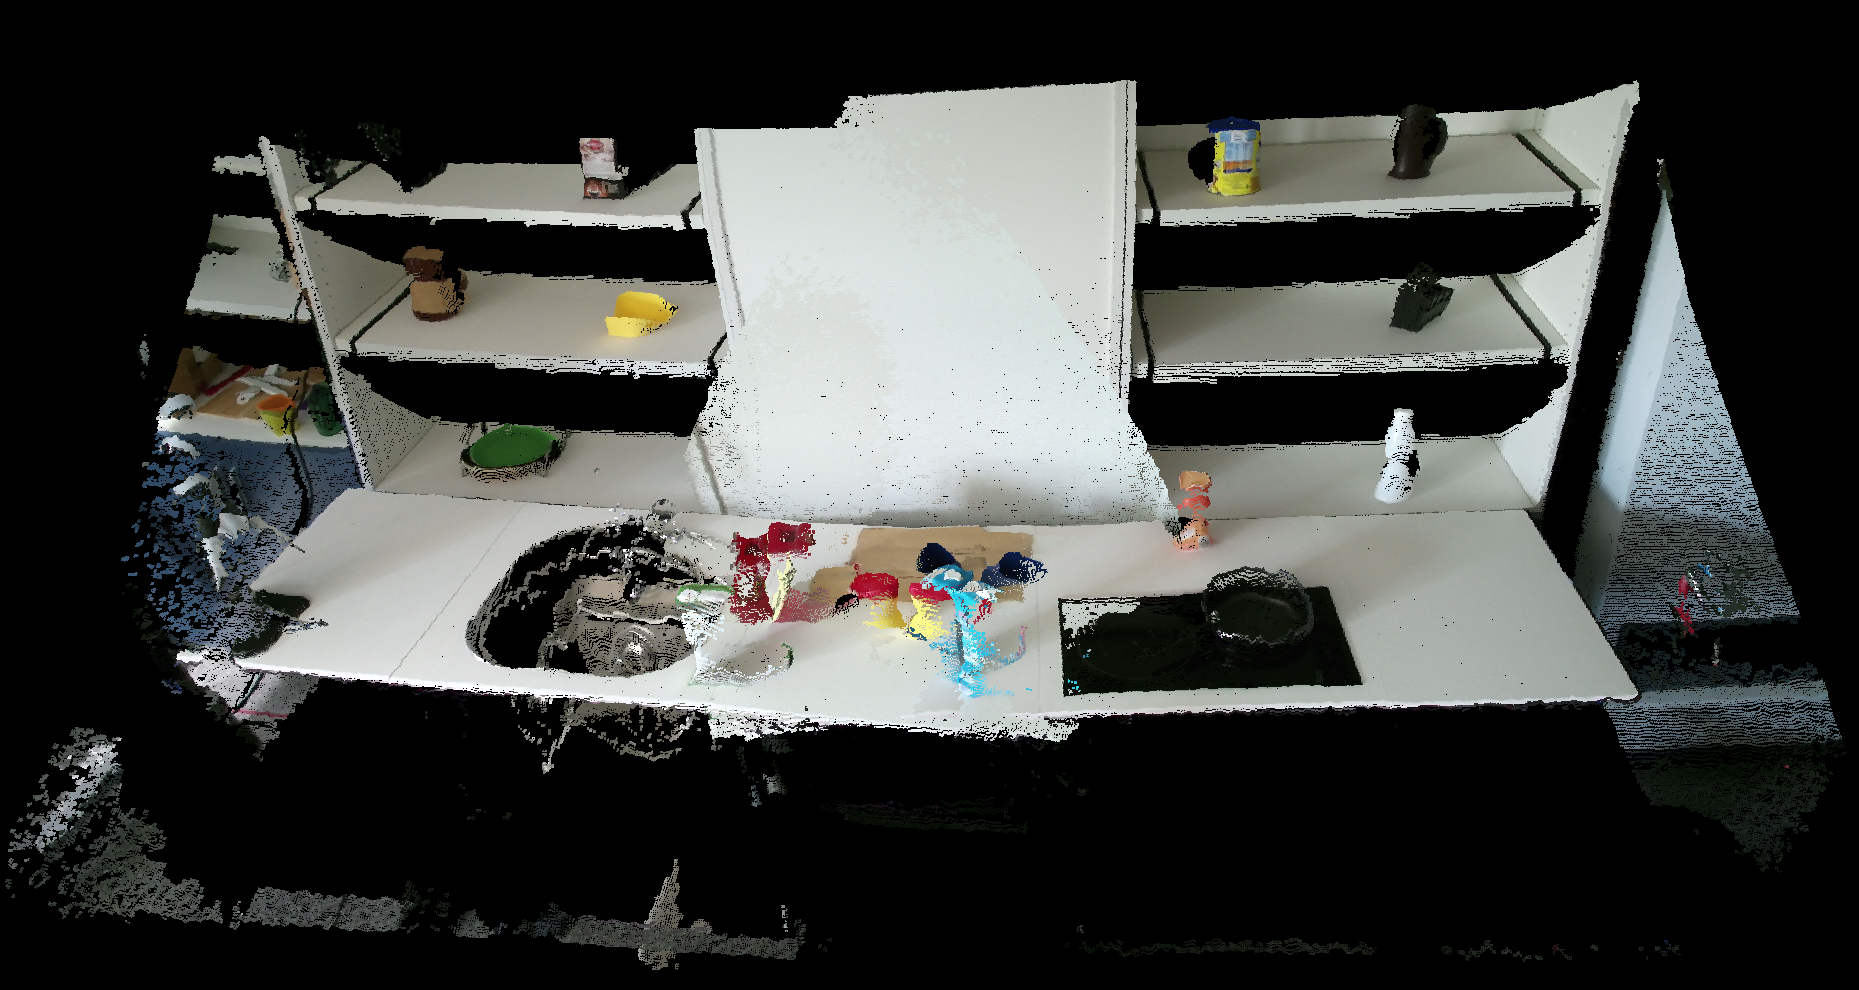
\includegraphics[width=\textwidth]{images/icp_one_one_registration.png}
    \caption{ICP applied to both cameras.}
    \label{fig:icp_cams}
\end{figure}

This algorithm is then useful when point clouds have a large overlapping or if we have previously built a model of the scene. As we are not assuming any knowledge on the environment (else than being indoor) and due to the low overlapping of our point clouds, this technique will not be used for the first registration of kinects. This can still remains a good registration method as soon as we have created a complete and reliable model of the scene.

% ***************************************************************************
\section{3D Keypoints}
% ***************************************************************************

An other commonly used registration technique consists in 3D keypoints detection and matching. There is a lot of different way tout compute features from keypoints but it basically consists in stacking 3D shape and/or color histograms into a vector descriptor, this descriptor can then be used to match the most similar keypoints to identify similar points (ie. that represent the same real point in space) from both clouds. This matching process means that this method is also relying only on overlapping regions to perform registration. The poor (size and quality) overlapping we have in this project will not allow me to use this kind of algorithm to perform the registration. \\
There are a lot of different ways to perform registration using 3D points matching, but the process pipeline is usually similar as the following:
\begin{itemize}
    \item Keypoints extraction: Input point clouds contains way to much points to run the entire process on all of them. It is thus required to select only a subset of them, we call these selected points, keypoints.
    \item Feature extraction: For each keypoint, we want to be able to find the most similar keypoint in the second cloud, it is then needed to describe the point in a way that is invariant to rotation (its equivalent point in the other cloud is probably oriented differently unless both clouds are yet aligned) and translation (scale invariant is not a property we are interested here since we assume cameras are calibrated). This description is usually based on geometric features (relative position or density of its neighbors) and/or color features (color distribution around the point).
    \item The next step consists in matching these descriptors, it basically consists in finding a coherent measure of distance within the chosen descriptor space so that a small distance between descriptors means that the corresponding points are similar.
    \item It is then often required to refine the previous matching by eliminating undesired matches such as if several points are matching with the same target point (we'll then keep only the best match, ie. with the smallest descriptor distance), called duplicates, points that are too far (in space) according to the initial guess or points with descriptor distance over a given threshold.
    \item The last step is then to estimate the transform that brings source matched points to their corresponding target points.
\end{itemize}

To apply this pipeline, I used the PCL implementation of these algorithms. I am using SHOT features which contains information on both geometry of the surrounding of the keypoint and color distribution. 
... \\
The resulting quality of this technique depends on matches accuracy (and successful matching ratio) but also on their spreading since the same error will produce a lower registration angle error if the keypoints matched are more distant. This, this algorithm will only be useful when a large part of the clouds is overlapping, in our case this method can't be applied.

% ***************************************************************************
\section{Plane detection}
% ***************************************************************************

An other interesting method that can be found in some papers is based on plane detection and matching. This method can solve the issue caused by low overlapping. Indeed, planes can be used to estimate how to merge the point clouds so that the overlapping region is continuous, but the interesting property is that the plane equation can be computed with every point that lies into the plane model whether it is in the overlapping region or not. Thus, if the cloud contains large plains that can be identified with a large number of points spread in a large part of the point cloud, the confidence on this plane's equation will be far better than if we try to identify features in the overlapping region. \\
However, to determine the whole 6 degrees of freedom of the transformation between camera positions, we would need 3 non-degenerate planes (ie. which normals describe a basis, the more orthogonal the better) to match in both point clouds. This condition is often too constraining to be satisfied, or is satisfied only if considering small and/or almost degenerate sets of planes. In this case, the accuracy gain provided by the plane identification is lost and one degree of freedom is left with a lot of uncertainty. Nevertheless, in most cases we can at least fix quite accurately the rotation between clouds (2 planes needed). \\
To apply this technique, I have used PCL's RANSAC implementation in order to achieve plane detection. Similarly to the previous registration method, the next step consists in matching extracted planes. \\
My first try was to match using feature matching in the same way as I did with keypoints descriptors but using global descriptors (descriptors that contains information on the entire plane). However, due to the similarity of planes in this particular scene (here, every planes is detected as an almost entirely white rectangle which fails the matching algorithm most of the time). Another technique could be to simply use brute force, since we are usually not trying to detect a lot of planes (we need 3 of them), by trying every possible matching we could make sure to keep the one that ends with the best registration result. Nevertheless this technique should better be applied to improve the matching after the whole registration process is implemented and optimized to reduce the computation speed, otherwise, repeating the process for every 6 matching possibilities may be too demanding. \\
For this reason I preferred to match planes by normal similarity, this technique doesn't rely on the later use of plane matches and is simple to implement. The only requirement is not to have a huge orientation difference between cameras. We may want to eliminate this assumption later but, for testing and comparison purpose, this method should be sufficient because it is highly reliable under this assumption and requires few computations. \\
The last step is to estimate the rigid transform that minimize plane-to-plane matching error as suggested in \cite{khoshelham2016}. 
\newline
If we define a plane as the vector $\pi=(n^T, -\rho)$ (normal vector and distance to origin) that satisfy for every point $p$ of this plane the equation:
\[\pi p=0\]
And let $H$ be the transform between point clouds A and B such that:
\[p^B = Hp^A\]
We can define $H'$ the transform that brings any plane equation in A $\pi^A$ to its corresponding plane in point cloud B $\pi^{B}$. We can demonstrate that: \[H'=H^-T\]
Finding $H$ is then the same as finding $H'$ that minimize plane distances: \[\pi^B_i=H'\pi^A_i\]
If we write:
\[H'=\begin{bmatrix}
R & t\\ 
0 & 1
\end{bmatrix}\]
We then have for each matching planes:
\[\left\{\begin{matrix}
{n_i^B}^TR={n_i^A}^T\\ 
{n_i^B}^Tt=\rho_i^B-\rho_i^A
\end{matrix}\right.\]
By stacking all $n$ vectors into a matrix $N$ and all $\rho_i^B-\rho_i^A$ into a vector $d$, the problem became:
\[\left\{\begin{matrix}
N^BR=N^A\\ 
N^Bt=d
\end{matrix}\right.\]
We can then simply compute the least square solutions for any n-dimensional distance metric where n is the number of matches. Especially, a useful metric could be for any n-d weight matrix $W$:
\[\mathcal{D}(x,y)=a^TWb\]
This metric will allow to weight some planes differently according to the confidence we give to the precision of their plane detection, otherwise $W=I_n$ will be used.
The final solution is:
\[\left\{\begin{matrix}
\tilde{t}=({N^B}^TWN^B)^{-1}{N^B}^TWd\\ 
\tilde{R}=({N^B}^TWN^B)^{-1}{N^B}^TWN^A
\end{matrix}\right.\]

At the end we can then ensure the orthogonality of $R$ using SVD decomposition. \\

The main limitation of this technique is that the scene needs to have large planes in it, but it is really common in indoor environments. However, having 3 large matching planes is lot more difficult, this is again an indirect consequence of the lack of overlapping. To identify 3 planes means that the sensor is seeing a corner but it is not probable being able to see this corner in both views if the overlapping is small, moreover even if we do, the corner will be in the border of both view, meaning at least one plane will be small. To summarize, we can't expect to detect required planes by luck. We may be able to use this algorithm in some specific cases but it is not possible to plan to use it if we don't have knowledge of the scene. 
\lhead{\emph{Methodology}}

% ***************************************************************************
\chapter{Methodology}
% ***************************************************************************

\section{Environment}

    As explained previously (\ref{int:chall}), the purpose of this work is to compare registration techniques in a specific case where point cloud registration is challenging. I realized a benchmark of methods described in the section \ref{ch:soa} and the modified one detailed in section \ref{chapt:implementation}. Each method is compared in different scenarios ; registering point clouds acquired from our real sensors in the kitchen scene, performing the registration on the kitchen with simulation data and finally with common point cloud databases to compare with the results from literature. 

    \subsection{Real scenario}

        Our real scenario is composed by 2 kinects filming a kitchen counter top and shelves filled with common kitchen objects. \\
        In this scenario on e of the main point is to define accurately the ground truth, is is possible to measure with few mm of error the translation between cameras but their relative orientation is much more difficult to measure. To evaluate this ground truth as accurately as possible I used all the knowledge we have: defining the initial guess as the manually measured translation and assuming equal orientation (cameras are facing in the same direction). I then align point clouds more accurately with the plane detection method and finely adjust the transform by hand so that point clouds match exactly.

    \subsection{Simulation}\label{subsec:simulation}
    
    Using 3D models of kitchen furnitures, I recreated the scene inside gazebo simulator which is compatible with \acrshort{ros} and I was able to publish point clouds topic using simulated kinects sensors. This setup is then working exactly in the same way as the previous one, our program can subscribe and share point cloud topics through \acrshort{ros}. \\
    In this case the ground truth is perfectly know as it is defined inside the gazebo world model where I placed the sensors with absolute coordinates and orientation.

\section{Variables}

    The objective of the algorithm is to estimate the transform between two kinects, I then need to compare this transform (rotation and translation) with the ground truth. It is difficult to find a meaningful scalar metric to compare transform matrices. We can nevertheless compare separately translation and rotation parts, by computing the overall translation distance $l$ and rotation angle $\theta$ around the fix axis $a$.
    Let $\mathcal{T}$ be the $4\times 4$ homogeneous matrix with rotation part described by coordinates of basis vectors $u, v, w$  the target frame written in the source frame and $t$ the translation vector between both frames' origins (fig. \ref{fig:transf}).
    \[
        \begin{bmatrix}
            u_x & v_x & w_x & t_x\\ 
            u_y & v_y & w_y & t_y\\ 
            u_z & v_z & w_z & t_z\\ 
            0 & 0 & 0 & 1
        \end{bmatrix}
    \]
    
    \begin{figure}[h!]
        \centering
        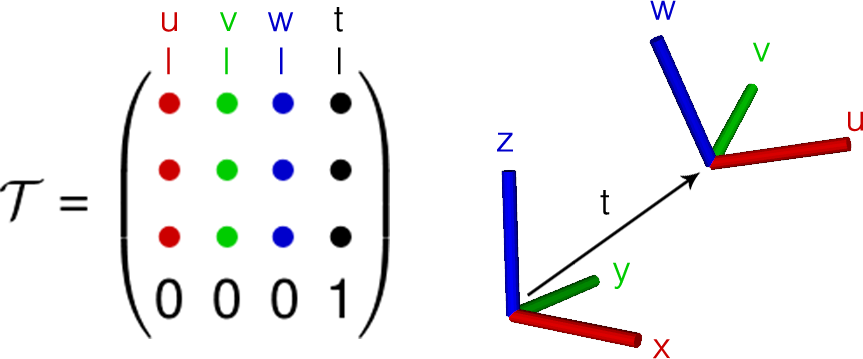
\includegraphics[width=\textwidth]{images/transform.png}
        \caption{Transform matrix description. \\
        $\mathcal{T}$ describes the transform between $xyz$ and $uvw$.}
        \label{fig:transf}
    \end{figure}
    
    We'll describe this transform with the following two metrics.
    
    \begin{equation} \label{eq:tf_transl_comp}
        \left.
        \begin{aligned}
        l(\mathcal{T}) &
        =   \begin{Vmatrix}
                t
            \end{Vmatrix} \\
         &
            = \sqrt{t_x^2+t_y^2+t_z^2}
        \end{aligned}
     \right\}
     \qquad \text{the translation metric}
    \end{equation}
    
    Using the fact that the rotation axis is 
    \[
        \mathbf{a}=\begin{pmatrix}
        w_y-v_z \\
        u_z-w_x \\
        v_x-u_y \\
        \end{pmatrix}^T
    \]
    with
    \[
        \begin{Vmatrix}
        \mathbf{a}
        \end{Vmatrix}
        =2sin(\theta)
    \]
    and 
    \[
        Tr(R) = 1 + 2\cos \theta
    \]
    We can compute the rotation angle from the matrix coefficients:
    \begin{equation} \label{eq:tf_rot_comp}
        \left.
        \begin{aligned}
        \theta(\mathcal{T}) &
        = \arctan \left( \frac{\sqrt{(w_y-v_z)^2 + (u_z-w_x)^2 + (v_x-u_y)^2 }}{u_x + v_y + w_z - 1} \right)
        \end{aligned}
     \right\}
     \qquad \text{the rotation metric}
    \end{equation}
 
\lhead{\emph{Implementation}}

% ***************************************************************************
\chapter{Implementation} \label{chapt:implementation}
% ***************************************************************************

All the above mentioned techniques appear to be efficient only under specific constrains. In our scenario none of them can be applied directly and we have to find a more suitable procedure for this project. \\
Even for humans, manually calibrating these point clouds is a hard task. Due to the lack of overlapping, it is difficult to notice whether a transform is wrong or not when focusing only on closest points matching (similarly to \acrshort{icp} algorithm). However, knowing that this is a scene containing large planes that can be seen in both views, we naturally tend to estimate the correctness of the registration by judging if the final result is coherent or not, if the planes are aligned or not (this is similar to plane matching). \\
Both this methods are used by our brain in the same time to evaluate how coherent is the matching. In the same way, our program have to mix both techniques to get the best result. Some similar approaches are described in the literature. The registration can be performed in one step, mixing keypoints (2D or 3D) and plane primitives as implemented in \cite{mdou2013} and \cite{ytaguchi2013} or in 2 steps \cite{pkim16}, in this case keypoints are used as a robust method to register 2 similar point clouds while plane matching is used in a second registration process to improve point cloud alignment. This 2 steps methods can't be applied to low-overlapping point clouds because, as explained in chapter \ref{ch:soa}, both methods can't be applied separately in this case.\\
\newline
As we have seen, the most reliable information we have is given by planes that are visible from both cameras. The first step would then be to identify as many planes as possible. Depending on how many planes we can match, the remaining degrees of freedom will be fixed with keypoints matching. \\
In this scene two mains plane can be identities, which means only one translation remains to be solved. Thus, only one point is needed, in theory, to solve the registration completely. The problem is that the point cloud quality doesn't let us find perfect matches. I will then try to identify as many matches as possible so that, on average, the error is lowered. \\
\newline
As explained previously, both registration using points matching or planes matching works in a similar way. It is still needed to adapt these equations to be able to find the transformation that minimize both points and planes distance in the same time. 

\section{Preprocessing}

Before implementing any registration technique, few preprocessing steps are required to prepare data, fasten computation and improve 

\subsection{Downsampling}

The first thing that appears is that point clouds are really heavy data structures and processing them will require a huge computation power. To be able to perform fast computation on point clouds I started by sub-sampling the point clouds to reduce the number of points.

\begin{figure}[h!]
\centering
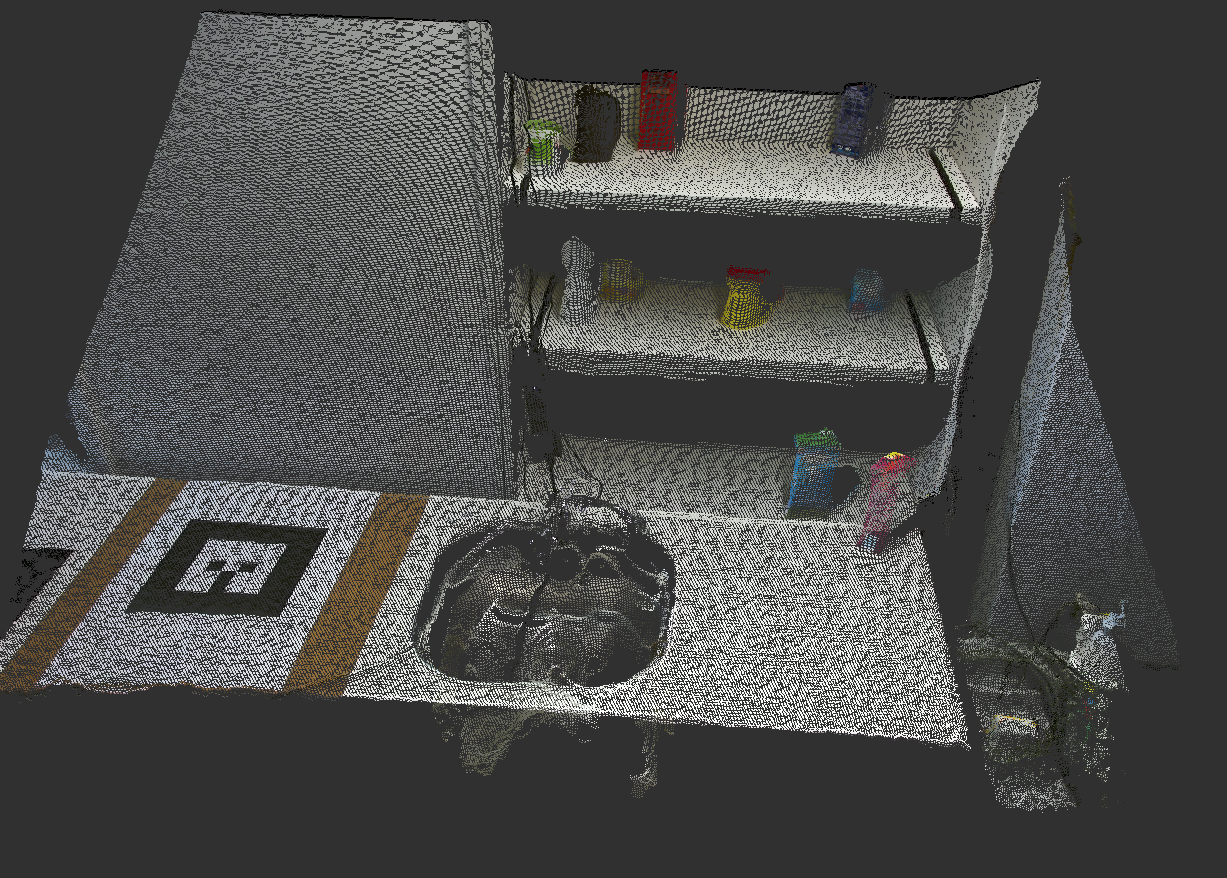
\includegraphics[width=\textwidth]{images/fullpc.png}
\caption{Full point cloud (16.588.800 points)}
\label{fig:fullpc}
\end{figure}

\begin{figure}[h!]
\centering
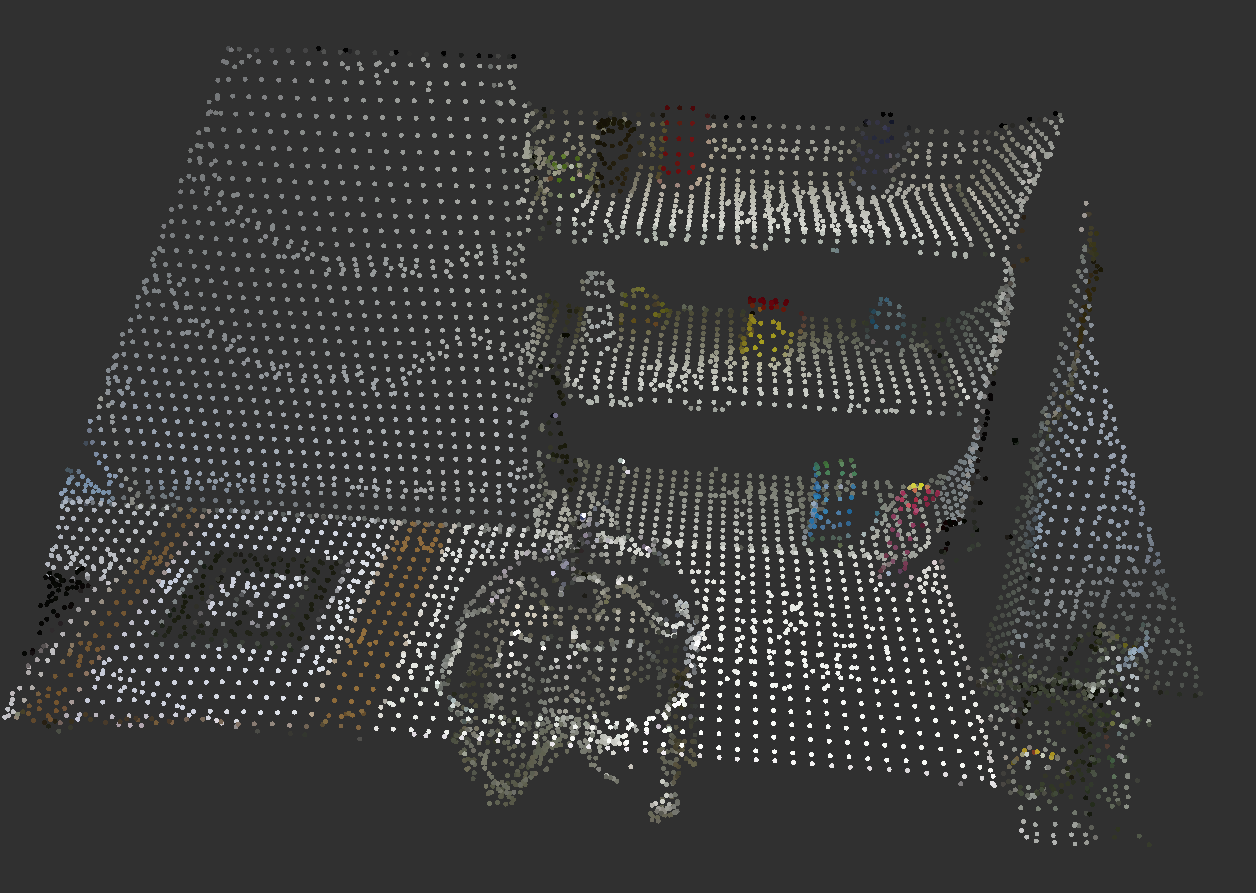
\includegraphics[width=\textwidth]{images/subsampled.png}
\caption{Sub-sampled point cloud (size: 3cm, 100k points)}
\label{fig:subpc}
\end{figure}

Sub-sampling allow to significantly decrease the size of the data to process by picking equally spaced points which makes the final result keeping most of the relevant information of the point cloud.

The sub-sampling size can be chosen to adapt the precision/performance ratio (fig. \ref{fig:sub_size}).

\begin{figure}[h!]
\centering
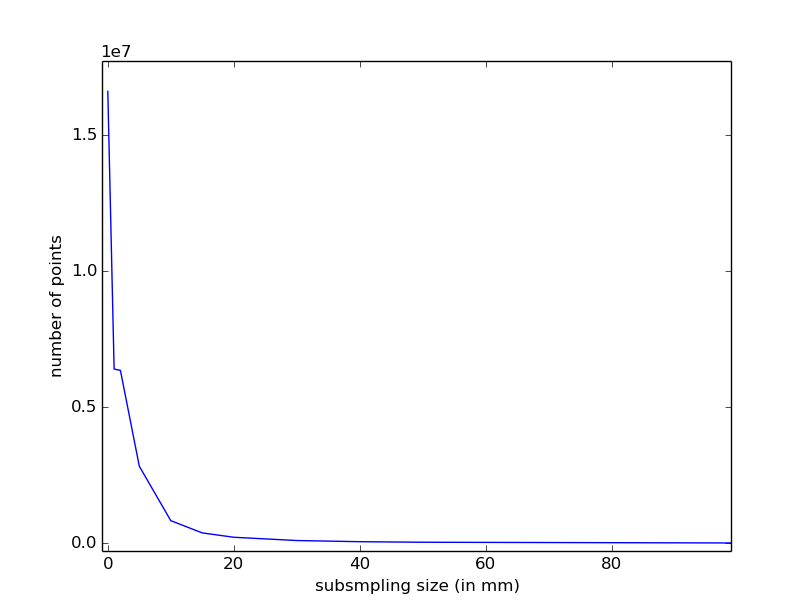
\includegraphics[width=\textwidth]{images/subsampling_size.png}
\caption{Example of evolution of the point cloud size against sub-sampling size.}
\label{fig:sub_size}
\end{figure}

\subsection{Cutting}

Another way to reduce the point cloud size is to cut it to remove non useful parts. This obviously requires to have some knowledge of the information received by the camera and will not be applicable in the case of a new unknown scene. However, cutting the point cloud will helps to quickly implement some registration techniques and will be used for testing and debugging purpose. In our project, when we try to fix only small camera displacements, we already have some rough knowledge on the scene. We can, for example, cut $z=0$ points that corresponds to the floor, using some margin threshold we can reasonably except that the floor will be cuted without losing any points on the table ($z=80cm$) unless the camera angle has been greatly modified.

\begin{figure}[h!]
\centering
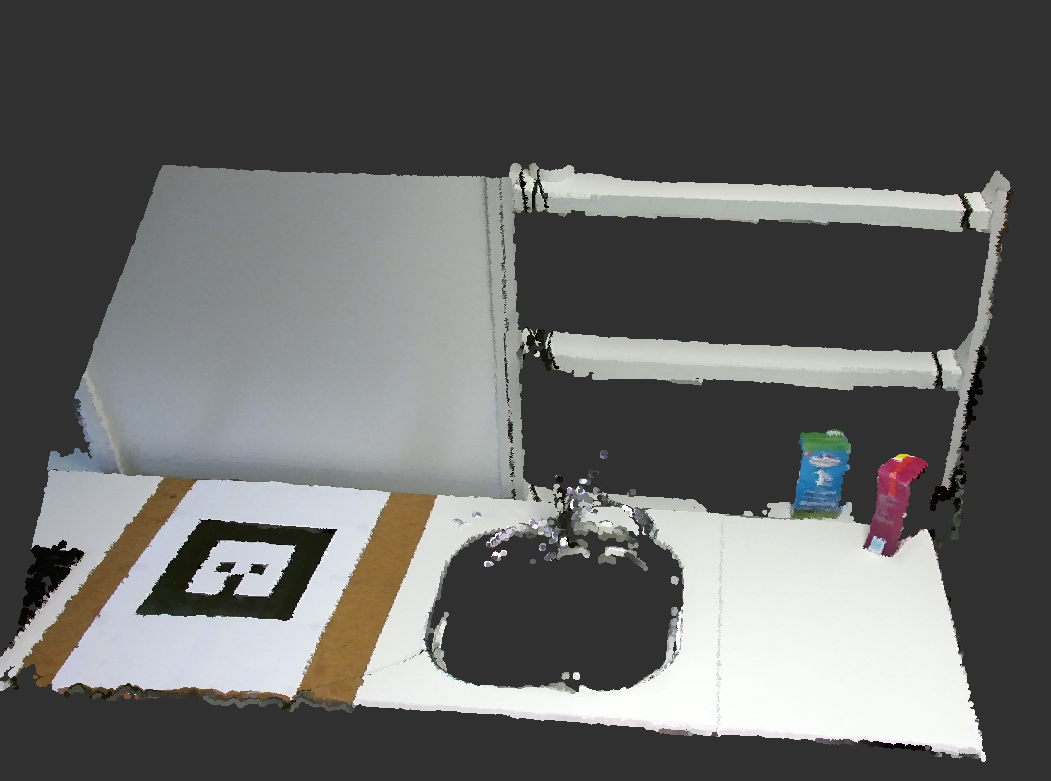
\includegraphics[width=\textwidth]{images/cut.png}
\caption{Example of point cloud cut using knowledge on the experiment environment.}
\label{fig:cut}
\end{figure}

In this example I cut the point cloud to keep only the points inside the working area.

\subsection{Filtering}

Finally, point cloud filtering is also a way I considered to decrease the size of the point cloud. I used radius filtering to delete outliers (points that don’t have enough neighbors inside a chosen radius). However this filtering was needing a lot of computation time compared to the small improvement it provides in this case. I no longer use this filtering in the preprocessing stage. 

\section{Plane Detection}

The first processing step consists in extracting planes from the point clouds. I am using \acrshort{ransac} (detailed in alg. \ref{alg:ransac}) algorithm to detect the most relevant plane of the cloud. I used \acrshort{pcd} \gls{library} implementation of this algorithm to perform fast plane detection.

When we find a good model, if we note $w$ the ratio between the number of inlying points and the total number of points, we can estimate the number of iterations needed to be confident enough that a correct model has been found. For example if we iterate the algorithm $k$ times, success probability $p$ can be written:
\[
    (1-w^3)^k=1-p
\]
The minimum number of iteration is then:
\[
    k=\frac{log(1-p)}{log(1-w^3)}
\]

In our setup, we can check how many iterations are needed. In the worst case, the first plane we want to detect is only $25\%$ of the point cloud. It means that using 500 iterations, we have less than $0.1\%$ chance not to find a good model. 

When the first plane is extracted, we can continue by subtracting inliers from the point cloud and apply again the \acrshort{ransac} algorithm, by iterating these steps I can extract as many planes as needed and they are extracted ordered by decreasing size. The idea is then to apply this plane detection on each point cloud in order to match these planes between both clouds. 

\section{Plane Matching} \label{sec:plane_matching}

Plane matching consists in matching as many planes as possible between different cameras. These planes should be matched when they correspond to the same plane in the real scene. Based on \cite{mdou2013}, I implemented a plane color histogram matching as follow. \\
By extracting the color data from each point of point cloud subsets corresponding to a plane we can compute a color histogram representing color distribution in a given color space. This space can be \acrshort{rgb} or \acrshort{hsv} and can be computer for 3 1D color channels (fig. \ref{fig:color_hist}) or for a 3D color space (fig. \ref{fig:3D_hist}).

\begin{figure}
   \begin{minipage}[t][6cm]{0.33\linewidth}
        \subfloat{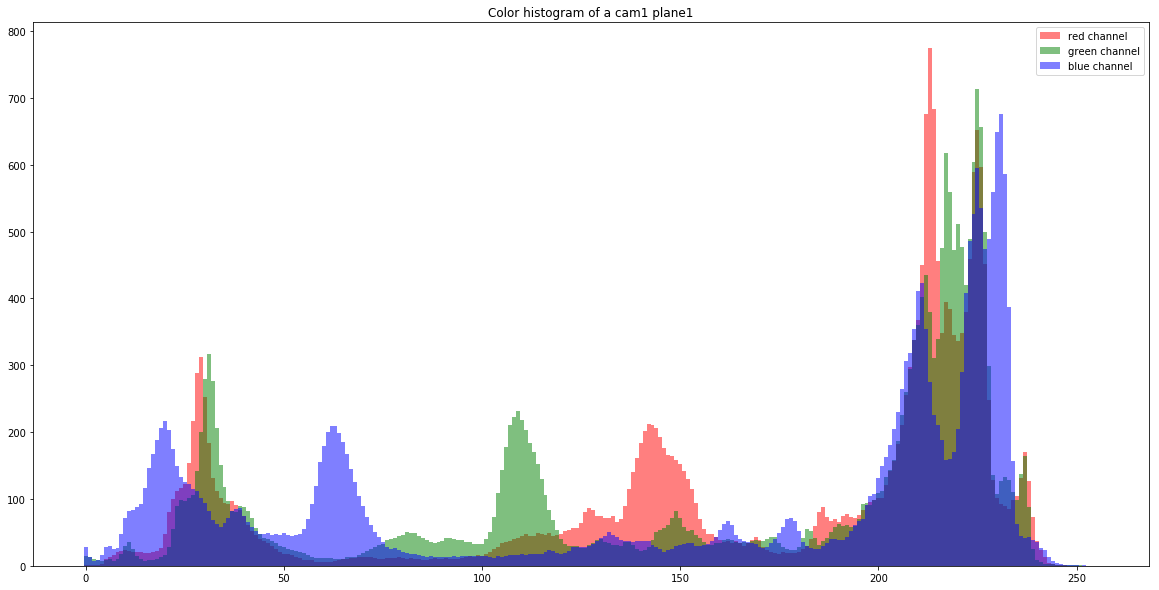
\includegraphics[width=\textwidth]{images/c1p1.png}}
        \subfloat{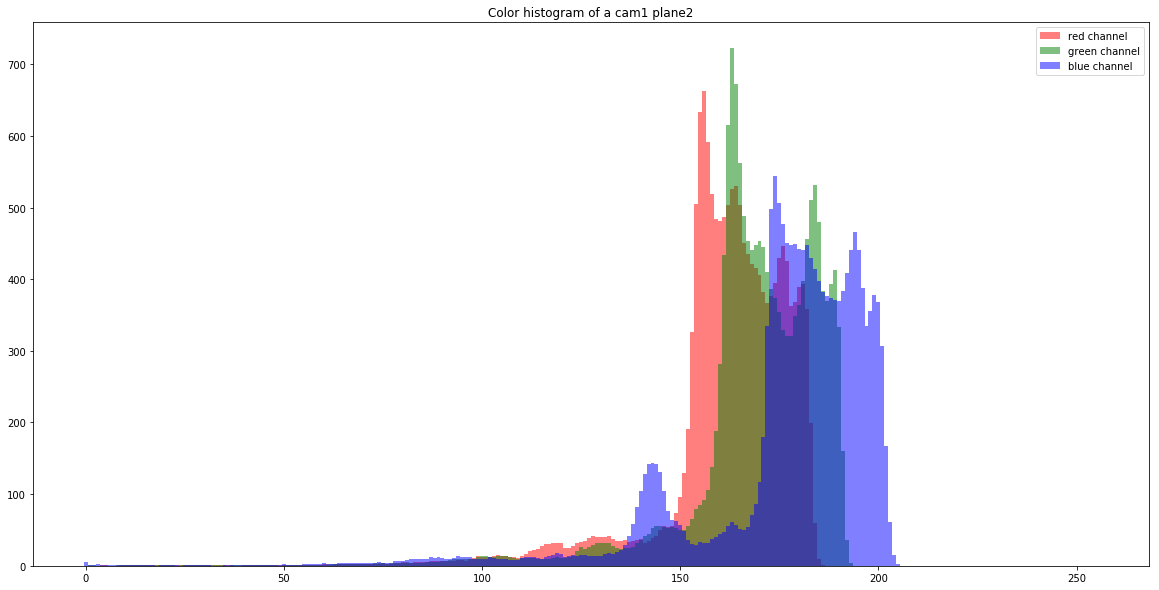
\includegraphics[width=\textwidth]{images/c1p2.png}}
        \subfloat{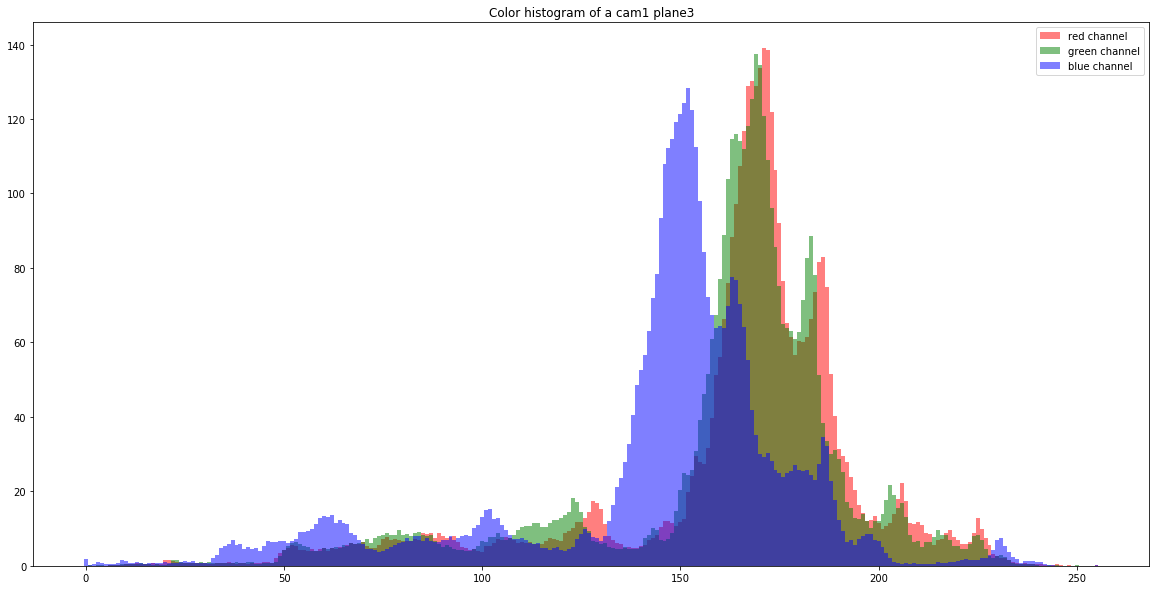
\includegraphics[width=\textwidth]{images/c1p3.png}}
    \end{minipage}%
    \begin{minipage}[t][6cm]{0.33\linewidth}
        \subfloat{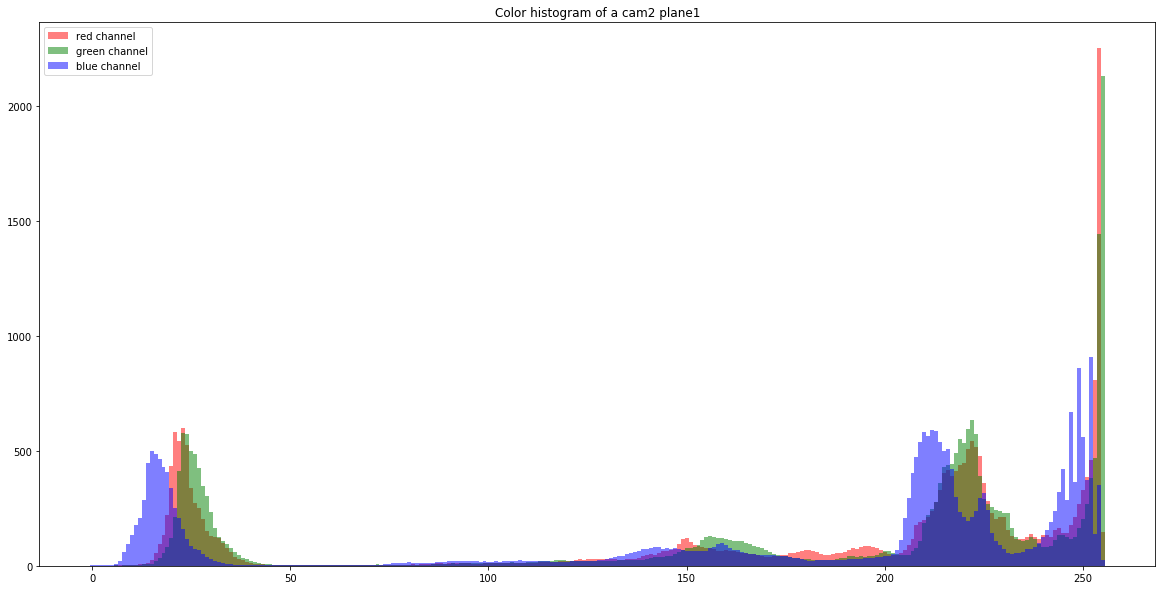
\includegraphics[width=\textwidth]{images/c2p1.png}}
        \subfloat{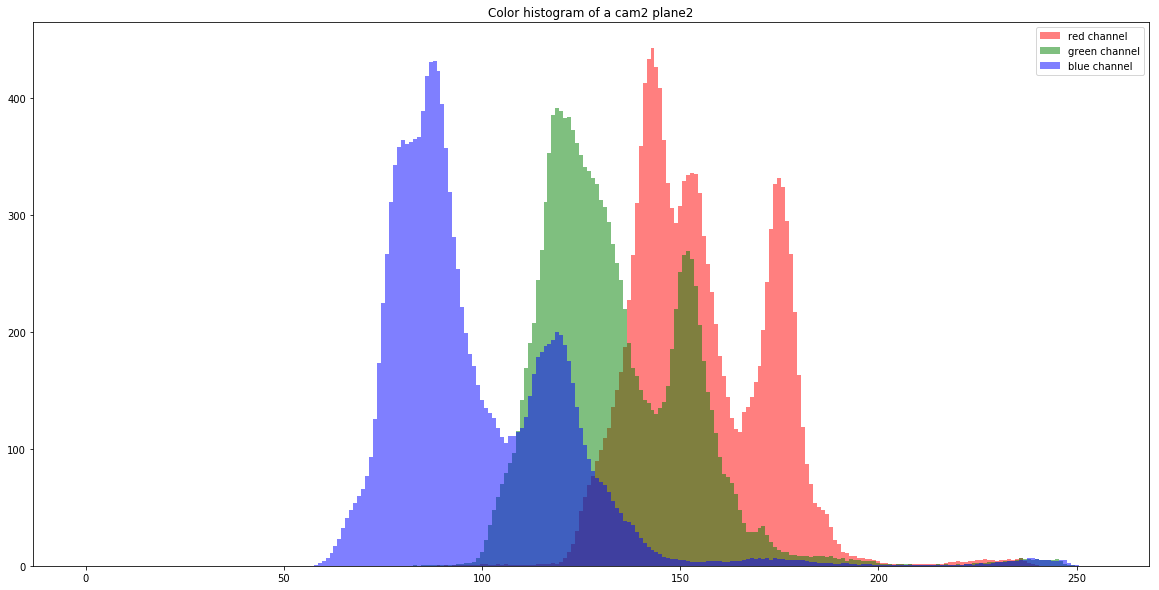
\includegraphics[width=\textwidth]{images/c2p2.png}}
        \subfloat{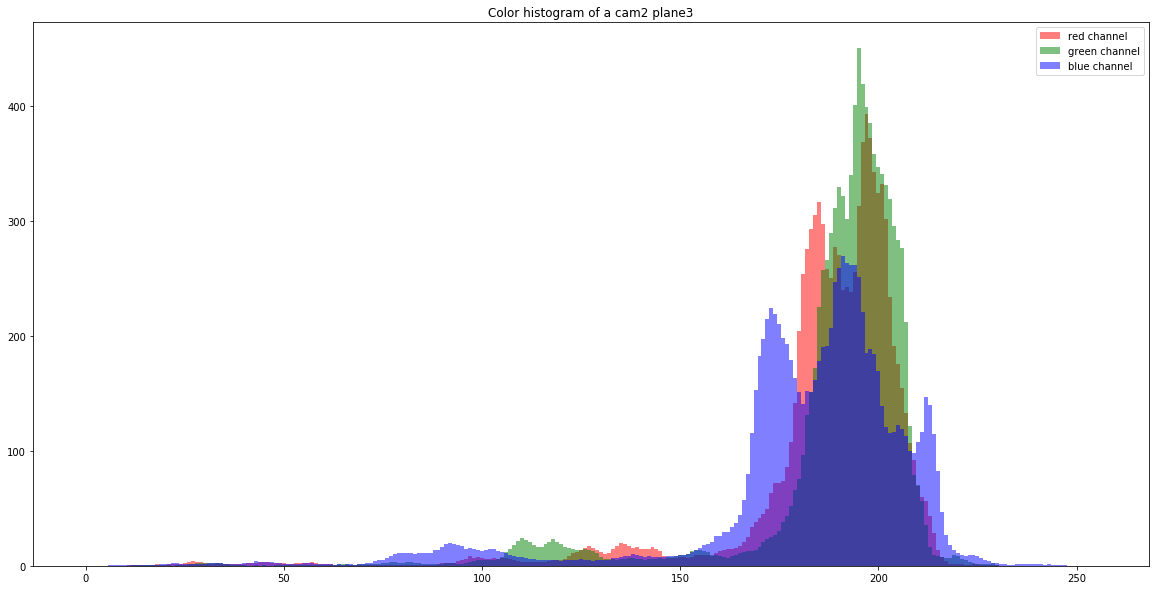
\includegraphics[width=\textwidth]{images/c2p3.png}}
    \end{minipage}
    \begin{minipage}[t][6cm]{0.33\linewidth}
        \subfloat{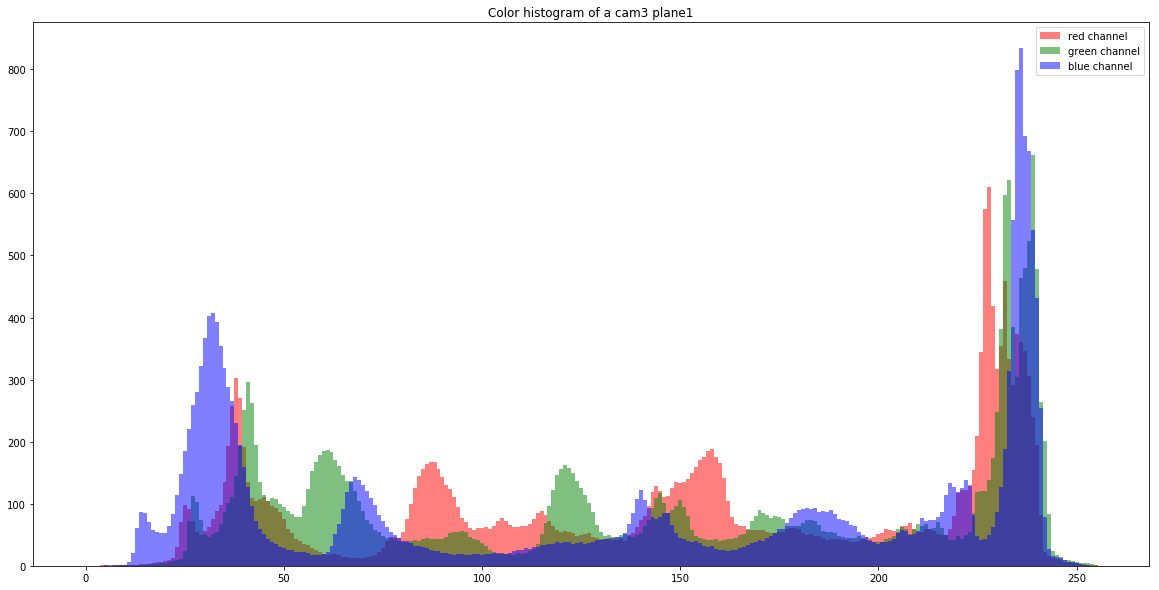
\includegraphics[width=\textwidth]{images/c3p1.png}}
        \subfloat{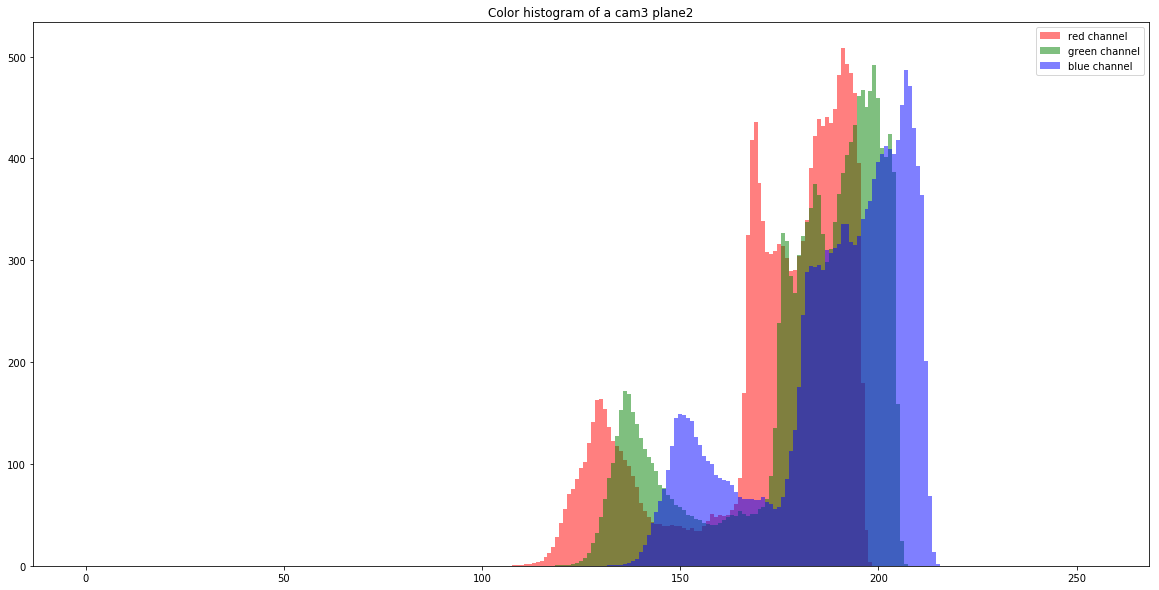
\includegraphics[width=\textwidth]{images/c3p2.png}}
        \subfloat{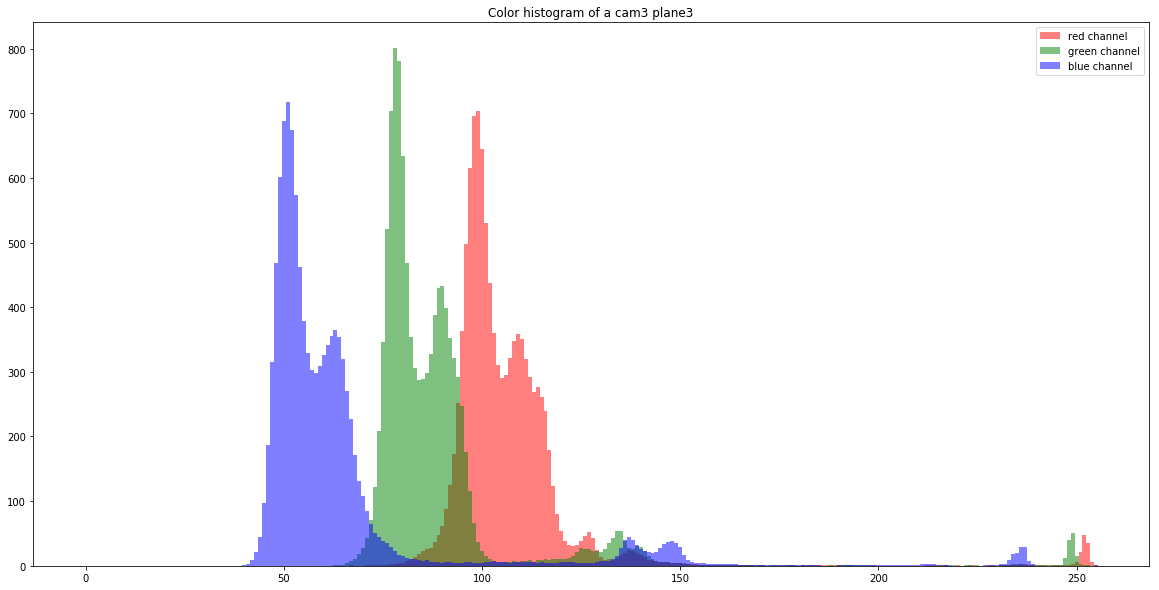
\includegraphics[width=\textwidth]{images/c3p3.png}}
    \end{minipage}
    \vspace{4em}
    \caption{Planes RGB color histograms computed for 3 cameras on 3 different planes (table, wall and wooden plate), each line represents a plane, each column represents a camera. }\label{color_hist}
\end{figure}

\begin{figure}[h!]
\centering
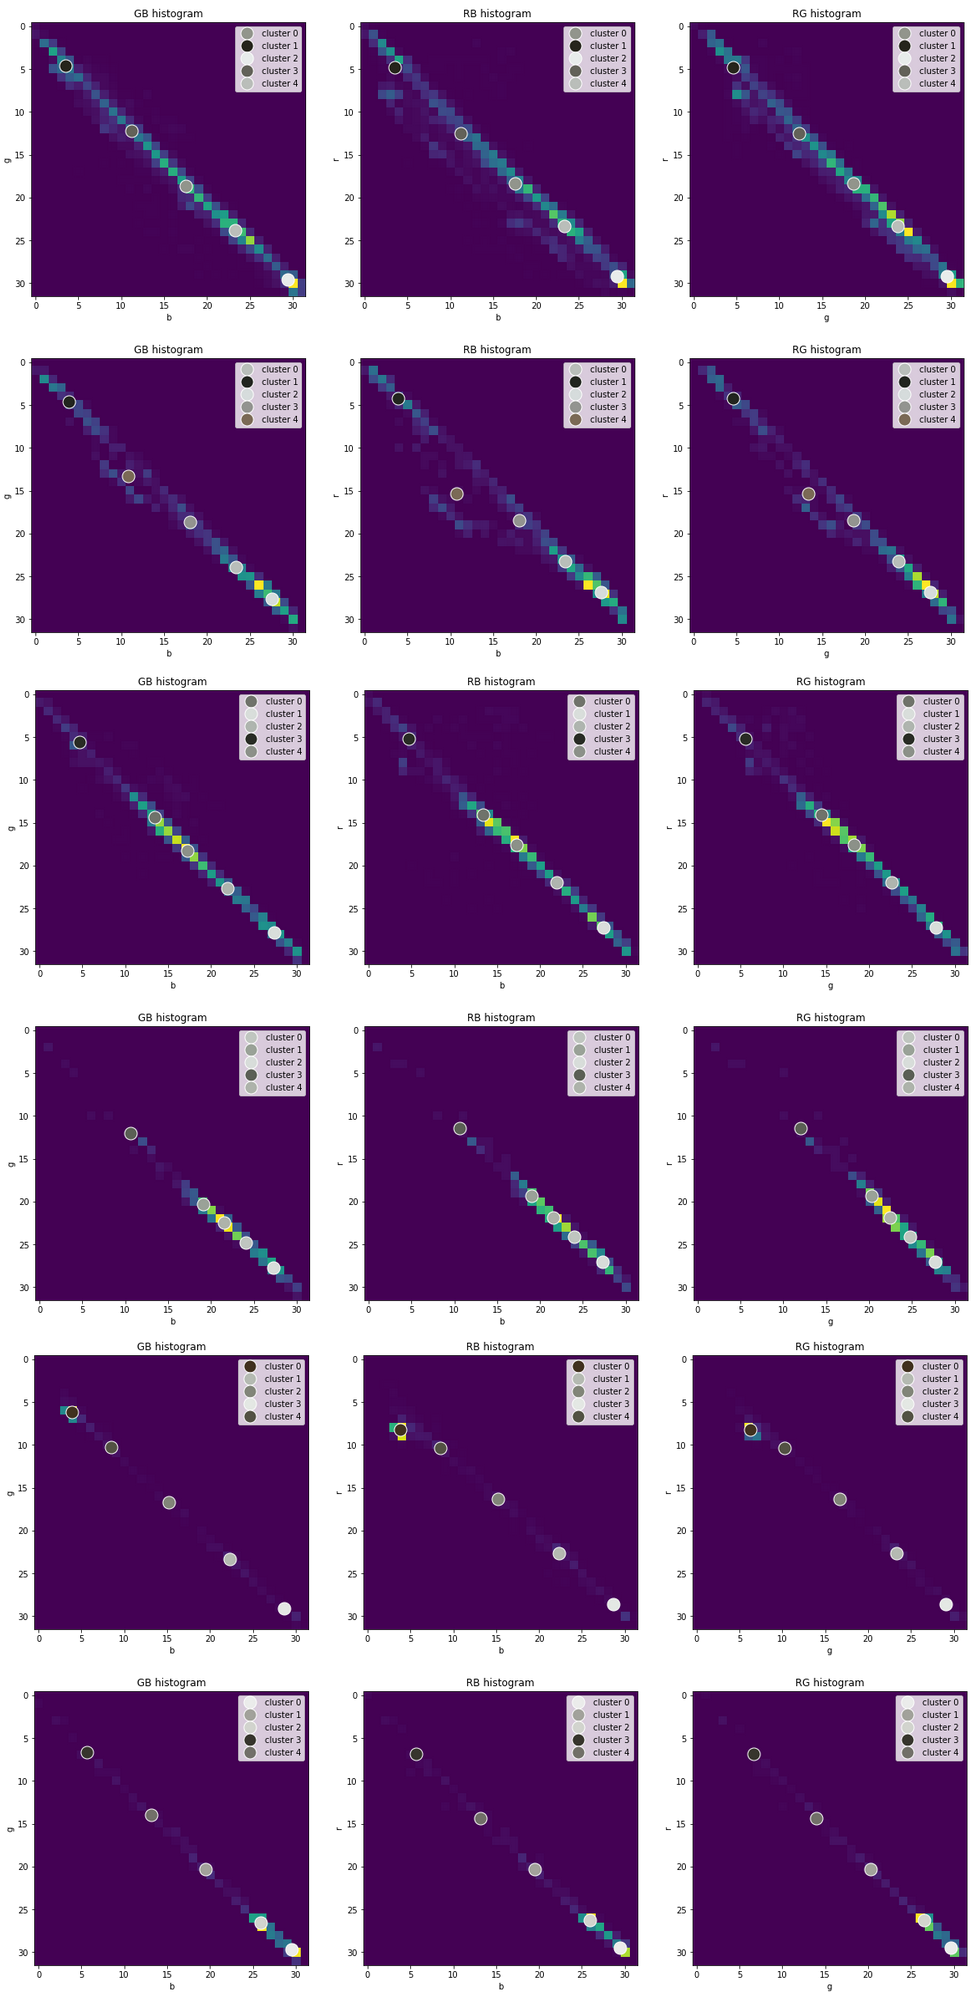
\includegraphics[width=0.8\textwidth]{images/kmeans_3D_hist.png}
\caption{2D projections of 3D color histograms for each planes. Lines correspond to plane 1 seen from cam1 (line 1) and from cam2 (line 2) then plane 2 (lines 3, 4) and plane 3 (lines 5, 6). Centroids of K-mean clustering (k=5) are shown with the corresponding color.}
\label{fig:3D_hist}
\end{figure}

Depending on the type of histogram different distance metrics can be used. As suggested in \cite{mdou2013}, overlapping areas can be computed for 1D histograms. I also performed K-means clustering on 3D histograms to determine the k=5 most common colors in each plane, it can be seen on fig. \ref{fig:3D_hist} that all colors are mostly grey which makes the matching difficult. It is then easy to compute a distance (Euclidian or Manhattan distance) between these centroids to find best matches. Given a plane color histogram from plane 3, I plot the distance to other planes color histograms captured from the 3 planes on both cameras on fig. \ref{fig:color_dist}. \

However, none of these techniques achieves a robust matching due to the very similar colors in each plane and the very low number of common points shared by planes seen from different cameras.
    
\begin{figure}[h!]
\centering
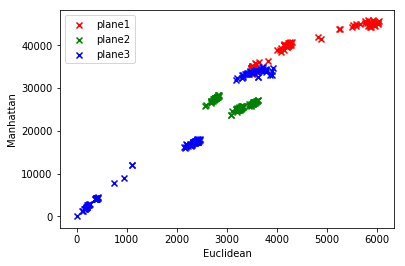
\includegraphics[width=0.6\textwidth]{images/dst_hist.png}
\caption{Distance between K-Means centroids computed between planes color histograms from different cameras and time and a color histogram from plane 3 seen from cam 1.}
\label{fig:color_dist}
\end{figure}



As explained in section \ref{sec:plane_detection}, I also tried to use \acrshort{pcl} \acrshort{vfh} global descriptor for matching planes. This techniques didn't allow me to match planes robustly neither.
For this reason, I preferred to match planes by comparing normals, this technique doesn't rely on the later use of plane matches and is simple to implement. The only requirement is not to have a huge orientation difference between cameras. This means we need a prior knowledge of the rotation between cameras ($\pm 45^\circ$). Given 2 planes $\pi_1=(n_1^\top, -\rho_1)$ and $\pi_2$ which normal vectors $n$ are chosen such that their product is positive, the metric $f$ I use for matching is the following, with an arbitrary $\alpha = 1\:m^{-1}$:
\[
    f(\pi_1, \pi_2) = n_1\cdot n_2 - \alpha \left | \rho_1 - \rho_2 \right |
\]

The first term $n_1\cdot n_2$ measures the cosine of normals angle between 0 (when they are perpendicular) and 1 (when they are parallel). The second term lowers this value if planes are far from each other. It allows planes to match with the right plane instead of an other parallel one.

\section{Keypoint Extraction}

As explained in sec. \ref{sec:plane_detection}, we usually don't detect 3 non-degenerated planes in the point cloud, especially when the overlapping is small. To solve this problem I am adding knowledge from the keypoints detection as done in \ref{sec:3dkp}. Method to estimate the transform from mixed data of planes and points is detailed in the next section.

Keypoints information is less precise than planes so we may want to give more importance to planes matching and use only keypoints to fix the last degree of freedom. We can define a weight between planes and points terms in the transform estimation equation. That way we give more importance to information provided by planes. However, we actually want to trust only planes for most of the degrees of freedom and use points matching only when it is needed. For example, we usually detect planes in 2 different orientations as we can see on fig. \ref{fig:planes_scene}, which means we still have to fix one degree of freedom (translation). We want, in this case, to use keypoints only to determine this translation. To achieve this, I compute the intersection direction of planes and I project keypoints along this vector. That way, keypoints will only contribute to modify the translation part of the transform in this direction as shown on fig. \ref{fig:proj}. By doing this we ensure that keypoints matching doesn't introduce a bigger uncertainty for rotations and translations that are already accurately determined by planes.

\begin{figure}[h!]
\centering
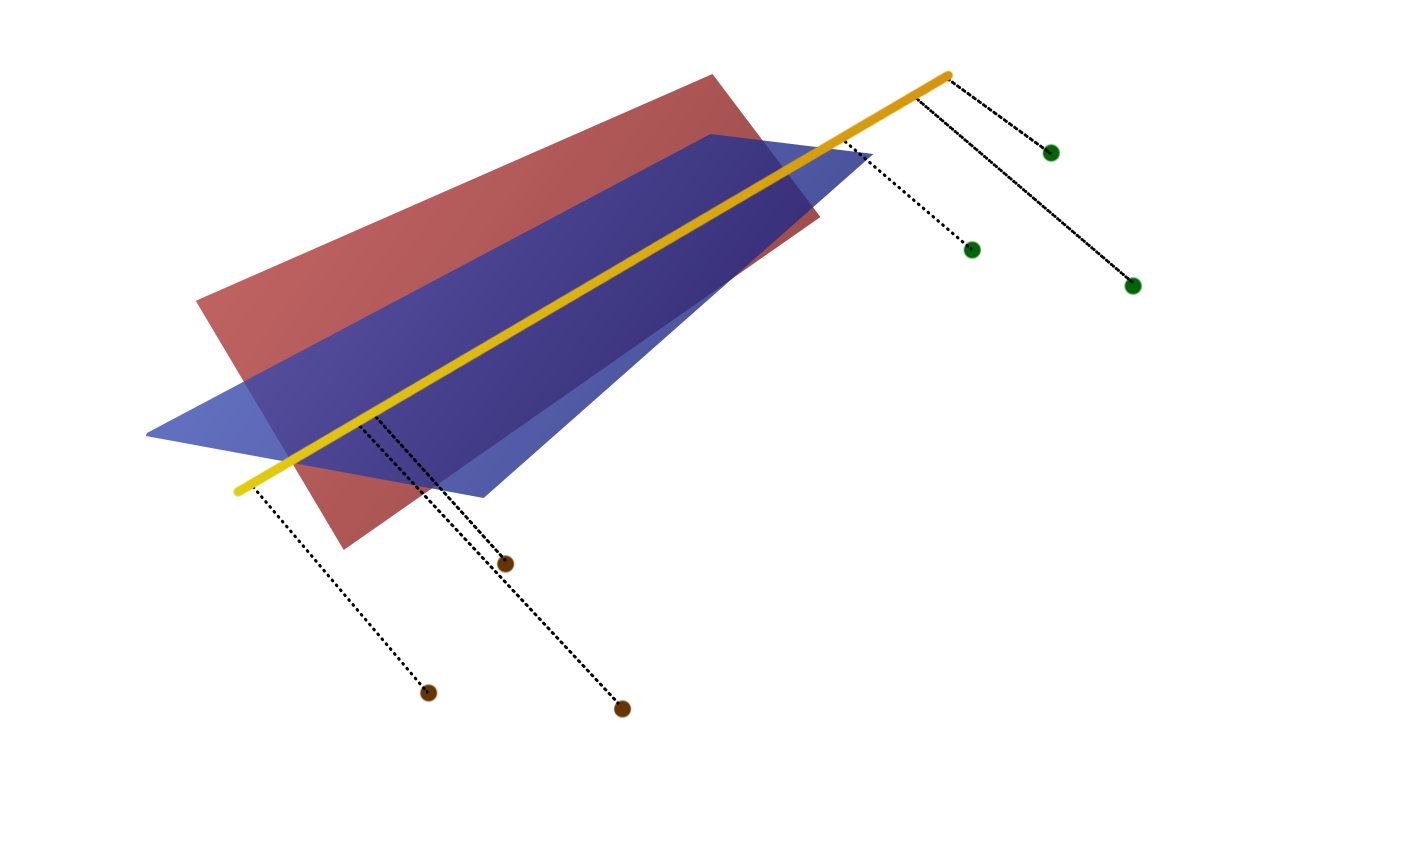
\includegraphics[width=\textwidth]{images/proj.png}
\caption{Projection of keypoints on plane intersection axis.}
\label{fig:proj}
\end{figure}

\section{Transform Estimation}

My implementation of transform estimation using both matched points and planes is based on equations derived in \cite{ytaguchi2013}. As described in \cite{khoshelham2016}, we can compute distances between planes (the value that should be minimized) in two different ways:

\begin{itemize}
    \item Plane to Plane, which is an arithmetic distance obtained by comparing plane equations. It is composed by the vector distance between plane normals and the scalar distance between $\rho$ parameters. 
    \item Point to Plane, a geometric distance obtained by averaging point to plane distances from one plane to another.
\end{itemize}

I am using the plane to plane distance since it is by far the fastest to compute.
My implementation is then based on these equations derived in \cite{khoshelham2016}. Equations are similar to the ones detailed in sec. \ref{subsec:transf_est} but we are adding terms (in red) related to plane normals. Resulting equations are then a generalized form of the equations from sec. \ref{subsec:transf_est} and \ref{sec:plane_detection}:

\[
R=U\begin{pmatrix}
1 &  & \\ 
 & 1 & \\ 
 &  & det(UV^\top))
\end{pmatrix}V^\top
\]
Where $U$ and $V$ are computed from the \acrshort{svd} of the $3\times 3$ correlation matrix $K$:
\[
K=UDV^\top=\sum_i p_i {p_i^s}^\top {\color{red}+ \sum_j w_j n^t_j n^s_j^\top}
\]

Where $w_j$ is the weight associated to planes with normals $n_j$ as defined in sec. \ref{sec:plane_detection} when $W$ is diagonal.

To compute the translation part we have to define $A$ and $b$:

\[
    A=\begin{pmatrix}
    MI_3 \\ 
    {\color{red} w_1n^t_1^\top} \\ 
    {\color{red} \vdots}  \\ 
    {\color{red} w_Nn^t_N^\top}
    \end{pmatrix}
\]
\[
    b = \begin{pmatrix}
    M(p'^t-Rp'^s)\\ 
    {\color{red} w_1(\rho_1^s-\rho^t_1)}\\ 
    {\color{red} \vdots} \\ 
    {\color{red} w_1(\rho_N^s-\rho^t_N)}
    \end{pmatrix}
\]

\[
    t = (A^\top A)^{-1}A^\top b
\]

\section{Program Description}

All these processing steps are run in separate \glspl{rosnode} and interact as explained on fig. \ref{fig:pipeline}

\begin{figure}[h!]
    \centering
    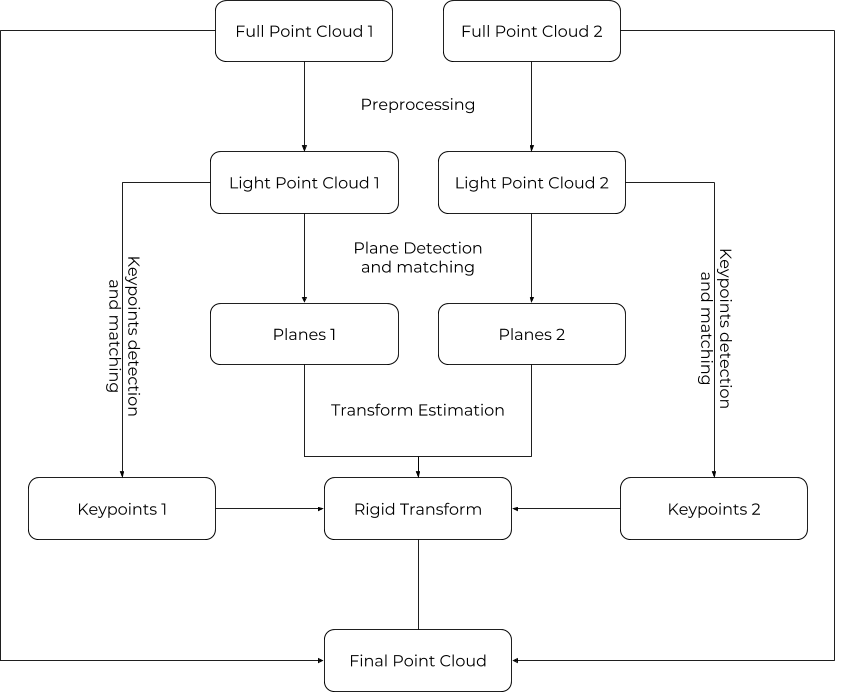
\includegraphics[scale=0.5]{images/pipeline.png}
    \caption{Registration pipeline.}
    \label{fig:pipeline}
\end{figure}

\lhead{\emph{Results}}

% ***************************************************************************
\chapter{Results}
% ***************************************************************************

\lhead{\emph{Conclusion}}

% ***************************************************************************
\chapter{Conclusion}
% ***************************************************************************

According to our results, this method mixing planes and keypoints matching leads to better results in this project. Indeed this method obtains the smallest error in translation over all the methods tested. For the rotation part, plane matching is performing as good as the mixed method in average (even slightly better but not significantly) but has a larger standard deviation. 
From these measures we can clearly see that matching methods (keypoints, planes and mixed) perform a lot better on this registration problem than ICP methods, 
\lhead{\emph{Future Work}}

% ***************************************************************************
\chapter{Future Work}
% ***************************************************************************

\section{Plane Matching}

\section{First Rough Transform Estimation}

\section{GPU implementation}


\clearpage
\printglossary[type=\acronymtype]
\listoffigures
\listoftables
\printglossary


\end{document}